\newpage
\section{电气总线选型设计}
\subsection{总体设计}
\subsubsection{架构分析}
在上一个部分,我们主要进行了机械总体概念设计以及具体模块的细节设计,在黑箱图\ref{hxt}中融合了机械运动、能量流动以及信息传递的几个通路,而以下就对整个AtomIC平台的电气部分绘制更为准确细分的拓扑图。主要功能架构如下:

\begin{figure}[htbp]
	\centering
	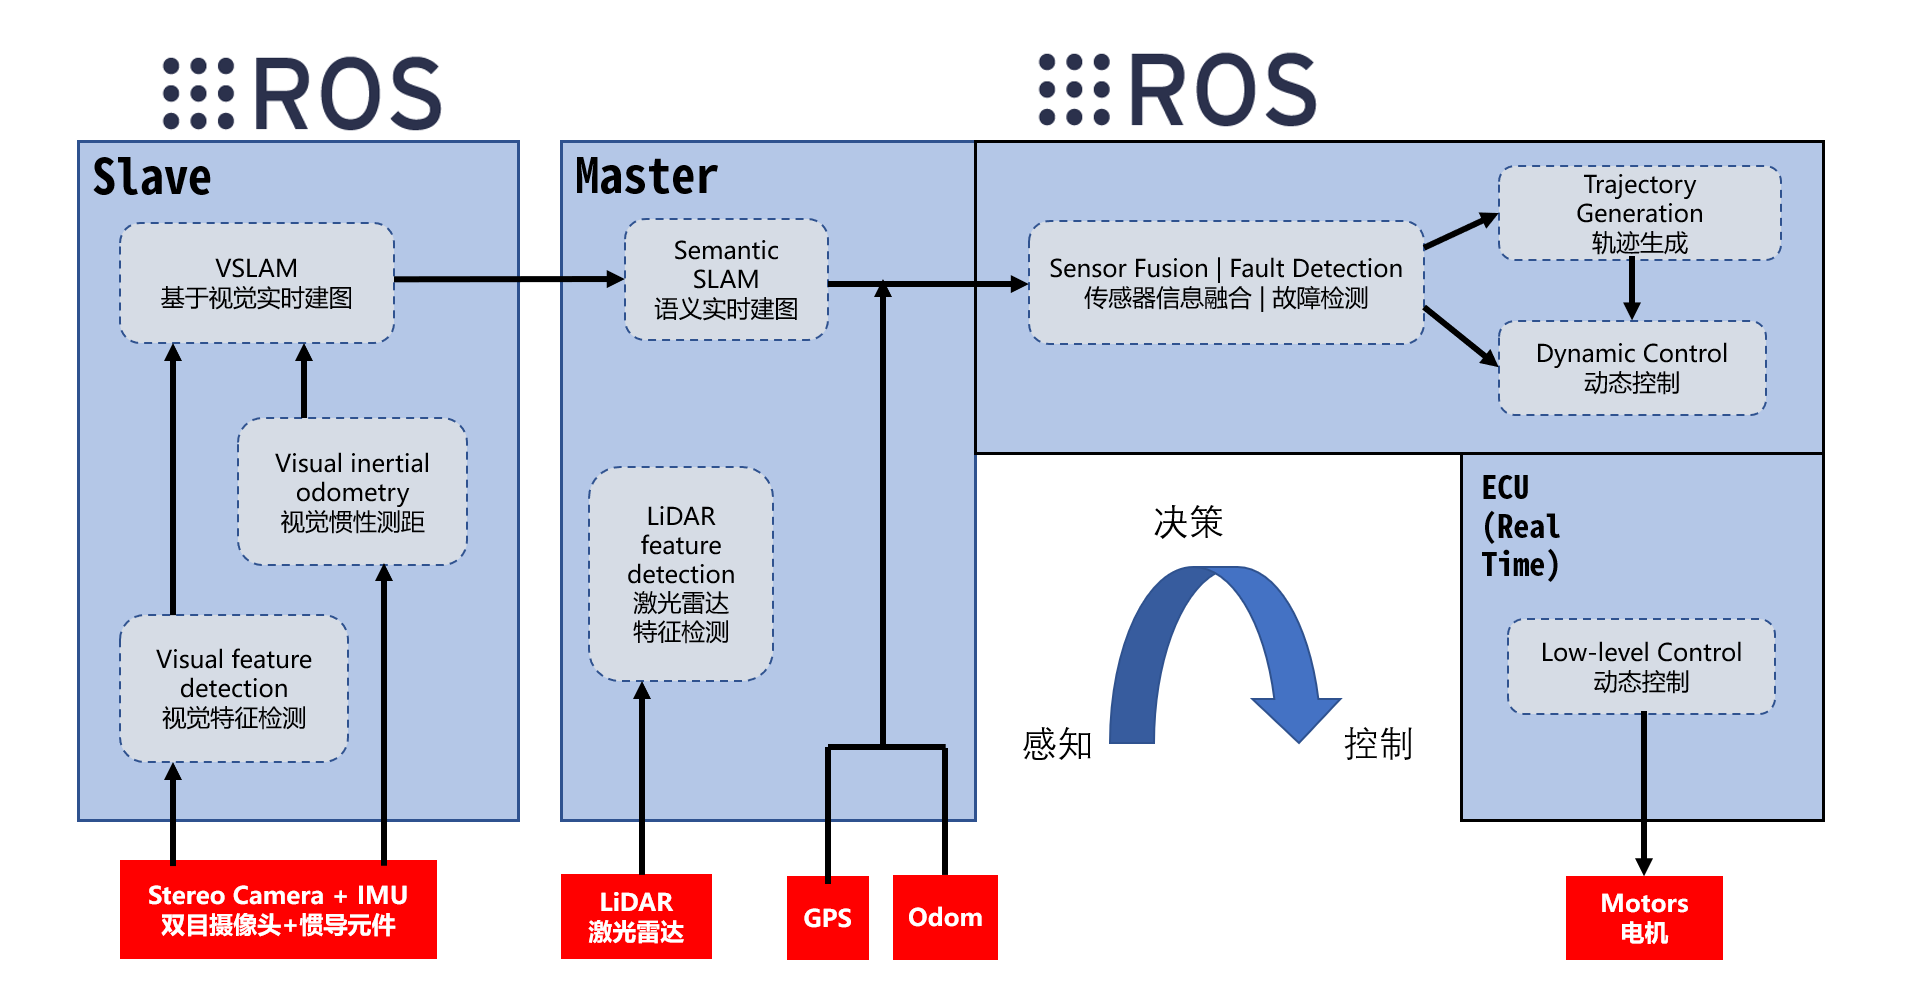
\includegraphics[width = 0.75\textwidth]{fig/rjjg.png}
	\caption{AtomIC功能框架}
	\label{rjjg}
\end{figure}

由上图可见,整体电气架构主要由\textbf{状态检测估计、三维建图、信息处理与决策、电机控制}四个主要部分组成。

\subsubsection{功能模块分析}

根据AtmoIC平台的功能,初步确定需要使用的电子元件,确定相关选型目标如下表\ref{dzdqxxmb}所示:

\begin{table}[htbp]
	\centering%表格居中
	\caption[centering]{电子电气选型目标}%表格标题
	\label{dzdqxxmb}%表格标签
	\begin{tabular}{C{3cm}C{3cm}C{6cm}}	
		\toprule
		\tabincell{c}{\textbf{功能}} &\tabincell{c}{\textbf{电子元件}} &\tabincell{c}{\textbf{通讯设备或协议}} \\ 
		\midrule
			\textbf{中心主控} & 开发计算平台 & CAN, UART, SPI, IIC, USB等\\
		    \textbf{底盘移动} & 直流无刷电机电调 & CAN或UART等\\
		    \textbf{三维建图} & 双目摄像头 & USB\\
		    & LiDAR & 以太网、USB等\\
		    & GPS   & CAN, UART, GPS, USB等\\
		    \textbf{自主避障} & 超声波模块 & GPIO等\\
		    \textbf{状态检测} & 陀螺仪 & IIC, RS232, CAN\\
		    & IMU & CAN, USB等\\
		\bottomrule
	\end{tabular}
\end{table}

\subsection{电子电气选型}

\subsubsection{传感器}

%—————————(1)图像传感器:LiDAR、双目摄像头——————————

\textbf{(1) 图像传感器}

根据经验,来自谷歌的工程师总结分析摄像头,LiDAR与radar之间的区别:

\begin{figure}[H]
	\centering
	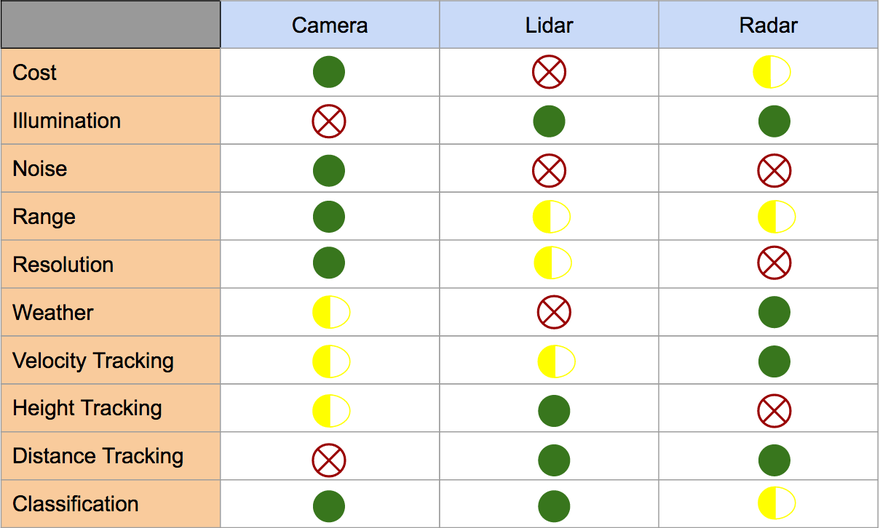
\includegraphics[width = 0.6\textwidth]{fig/shijueyj.png}
	\caption{摄像头,LiDAR与radar的区别分析}
	\label{shijueyj}
\end{figure}

相关解读如下:

\textbf{价格:} 相对于动辄几万的lidar和radar,摄像机较为便宜便宜的;但一般毫米波radar相对高精度激光雷达差距较大

\textbf{照明影响:}摄像机在不同的光照条件下的性能是非常不一样,尤其是无人车在道路上快速移动的时候。相比较而言,激光雷达和雷达的作用就彰显出来了。 他们在感知周围环境的时候,不受任何光照影响。所以在光照条件不好的情况下,在感知层面上系统会给来自lidar和radar的数据更高的权重。

\textbf{噪声影响:}在这个方面,lidar和radar在传达数据时候的时候,受到电路的影响,从而获得的噪声。

分辨率:相机最高,Lidar次之,Radar最低

抗天气影响能力:Radar最好,Camera次之,Lidar最低

追踪物体速度能力:Radar最好,Camera和Lidar差不多

追踪距离能力:Lidar,Radar都很准确,Camera最低

辨别能力:Camera和Lidar都较好,Radar较低。

作为一个自动化底盘,以实验为目的,以特定场景为主攻对象,因而暂时确定为LiDAR与双目摄像头综合的方案,除开价格因素,目前在应用自动驾驶领域较为广泛,相关基础需求如下所示:

\begin{table}[H]
	\centering%表格居中
	\caption[centering]{图像传感器需求}%表格标题
	\label{txxq}%表格标签
	\begin{tabular}{C{2cm}C{3cm}p{3cm}p{4cm}}	
		\toprule
		\tabincell{c}{\textbf{传感器}} &\tabincell{c}{\textbf{工况}} &\tabincell{c}{\textbf{功能}} &\tabincell{c}{\textbf{注意事项及要求}}\\ 
		\midrule
		
		\textbf{LiDAR} & 1个,布置于前部 & 用于激光雷达发射接收用于三维建图 & 尺寸要尽量小且比较轻;线束继承便于稳定通信 \\
		\\
		\textbf{双目摄像头} & 1个,布置于云台 & 信息采集用于三维建图 & 尺寸要尽量小且比较轻;应有相关封装 \\		
		
		\bottomrule
	\end{tabular}
\end{table}

\begin{figure}[H]
	\centering
	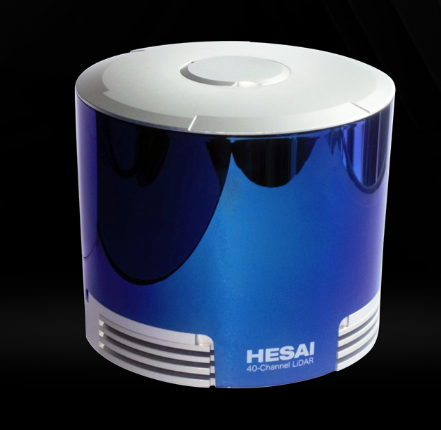
\includegraphics[width = 0.3\textwidth]{fig/LiDAR.png}
	\caption{Hesai Pandar40 LiDAR外观}
	\label{LiDAR}
\end{figure}

\textbf{LiDAR}确定为\emph{Hesai Pandar40 40线混合固态激光雷达}。它属于飞行时间测量法(Time of Flight) 测距方式激光雷达,通过内部旋转电机进行360度激光测距,共有40线激光分布,主要支持USB,以太网,CAN等总线通信协议。
主要由激光雷达和接线盒两部分组成,如下所示。

\begin{figure}[H]
	\centering
	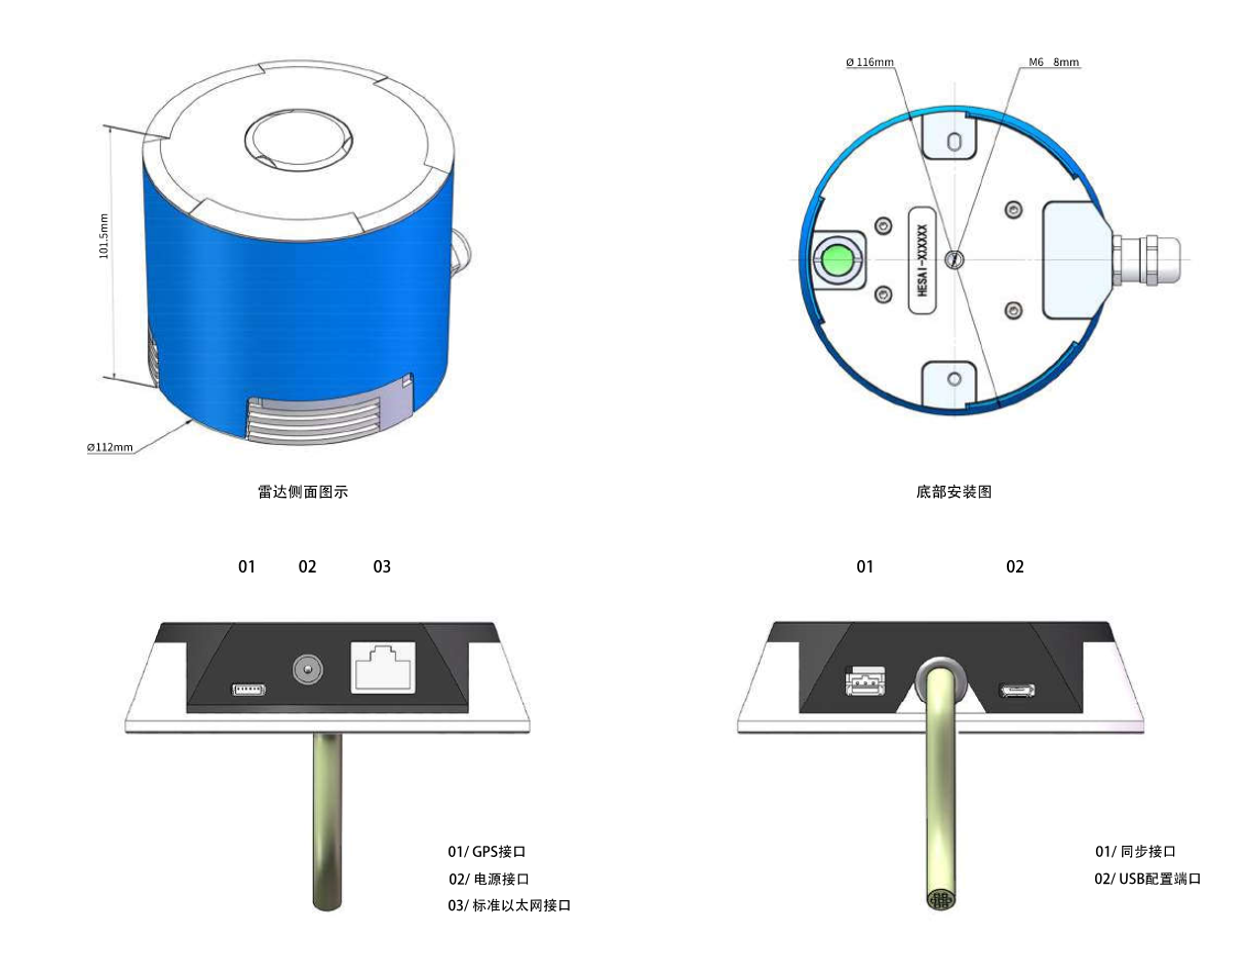
\includegraphics[width = 0.5\textwidth]{fig/LiDAR_IO.png}
	\caption{Pandar40 LiDAR主体及其接线盒示意}
	\label{LiDAR主体及其接线盒端口}
\end{figure}

上述左图中的[1]端口所表现的6线GPS与Pandar40之间采取UART串口通信,上述右图中的[1]端口为Pandar40的数据传输线,采用以太网UDP/IP通信协议。使用PC端测试可以按照如下流程:

\begin{figure}[H]
	\centering
	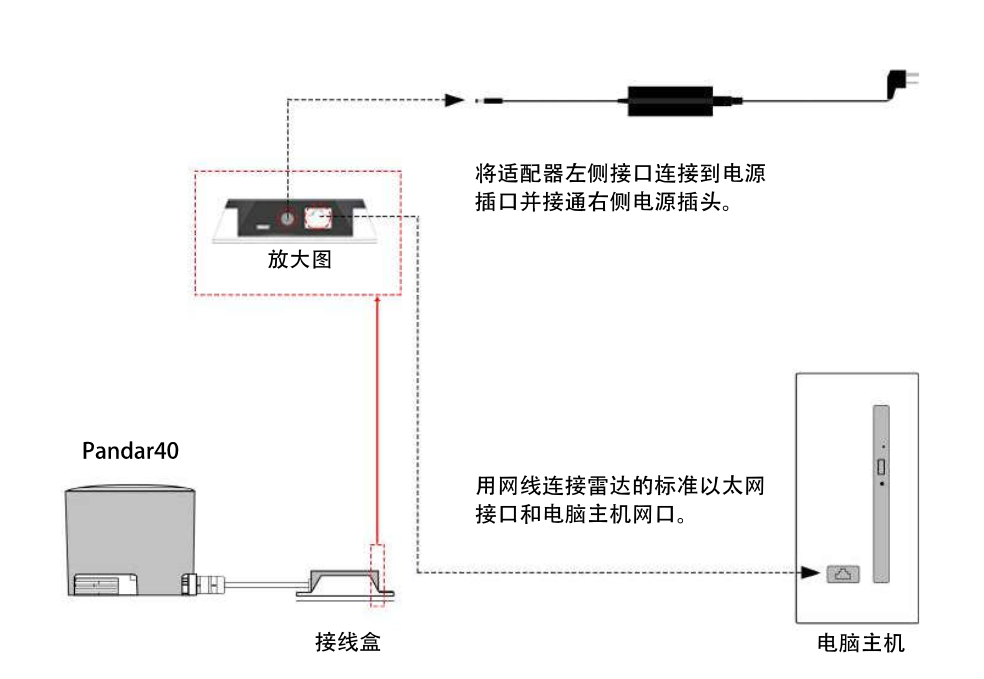
\includegraphics[width = 0.5\textwidth]{fig/LiDAR_test.png}
	\caption{Pandar40 LiDAR 测试接线方式}
	\label{LiDAR_test}
\end{figure}

由产品手册总结得出,对于在线LiDAR点云信号处理流程如下所示:

\begin{figure}[H]
	\centering
	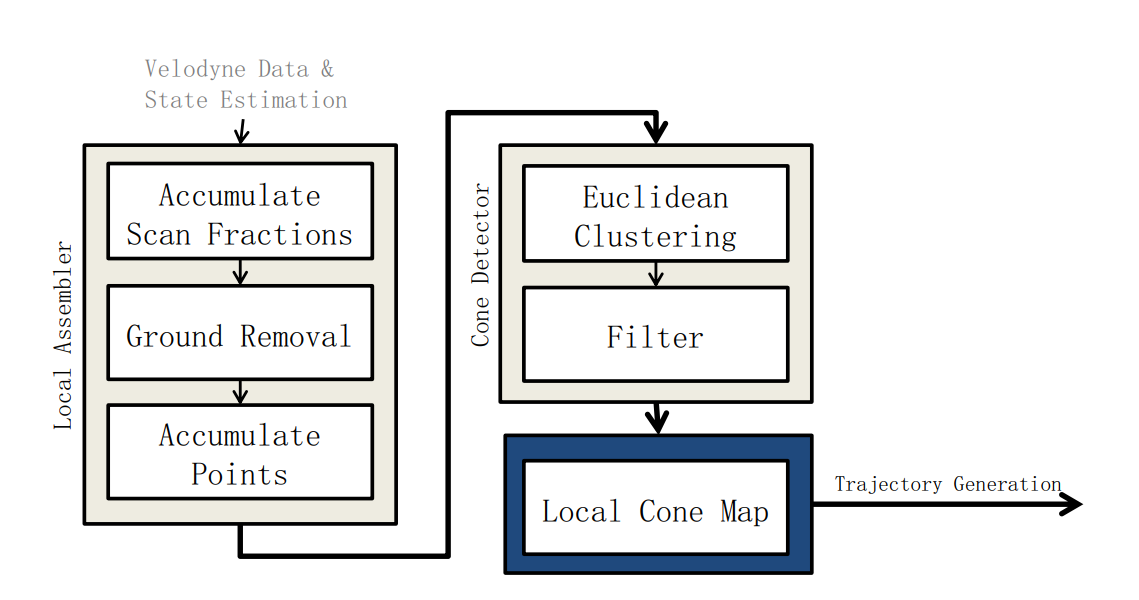
\includegraphics[width = 0.6\textwidth]{fig/LiDAR_pipeline.png}
	\caption{LiDAR信号处理流程}
	\label{LiDAR_pipeline}
\end{figure}

%LiDAR确定为\emph{Alubi LPMS-CANAL2}。它属于精尖MEMS 微型惯性测量单元;集成三轴陀螺仪、三轴加速度计、三轴磁力计、 气压传感器;实时计算传感器的姿态方向、线性加速度以及海拔高度等数据,主要通信接口为CAN Bus。

相机是视觉建图核心的部件之一。选型时需要考虑的点有这么几个: 分辨率(Resolution); 视场角(Field of View);基线长度(Baseline);视场角(Field of View); 曝光方式(Shutter); 帧率(Frame Rate)

不考虑价格的话,帧率肯定是越大越好,但是考虑到对高帧率相机、 计算单元价格的妥协,一般情况下 30f/s、 60f/s 即可。这里主要是取决于目标运动速度。 通讯方式:因为相机传出来的图像还需要进行处理,因此相机应该尽可能配备更加丰富的接口。综合考虑价格和以上性能指标,双目摄像头确定为\emph{ZED}。它属于精尖MEMS,其主要通信接口为USB, 同时采用USB 5V 380mA供电。相关参数为最大视场为90° (H) x 60° (V) x 110° (D)。

\begin{figure}[H]
	\centering
	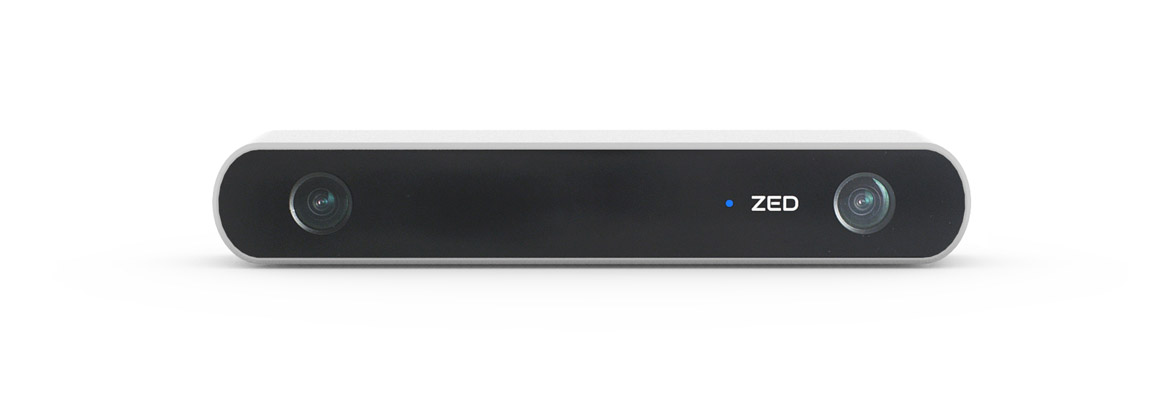
\includegraphics[width = 0.5\textwidth]{fig/zed.jpg}
	\caption{Stereolabs ZED双目相机外观}
	\label{zed}
\end{figure}

结合LiDAR与双目摄像头的最终选型及安装示意如下图:

\begin{figure}[H]
	\centering
	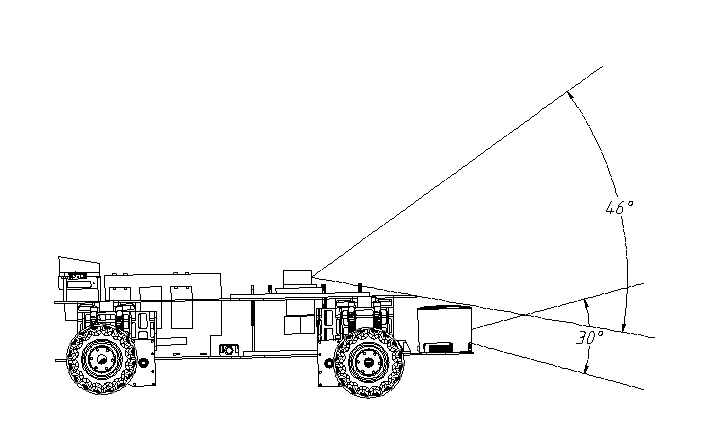
\includegraphics[width = 0.6\textwidth]{fig/sjyj.png}
	\caption{图像传感器视场示意图}
	\label{sjyj}
\end{figure}

%——————(2)运动参数传感器:陀螺仪、光学————————————————————

\textbf{(2) 运动参数传感器}

相关基础需求如下所示:

\begin{table}[H]
	\centering%表格居中
	\caption[centering]{运动参数传感器需求}%表格标题
	\label{ydxq}%表格标签
	\begin{tabular}{C{2cm}C{3cm}p{3cm}p{4cm}}	
		\toprule
		\tabincell{c}{\textbf{传感器}} &\tabincell{c}{\textbf{工况}} &\tabincell{c}{\textbf{功能}} &\tabincell{c}{\textbf{注意事项及要求}}\\ 
		\midrule
		
		\textbf{陀螺仪} & 1个,布置于车身重心 & 测量三轴角加速度、加速度,作为动态控制算法的必要参数 & 供电电压必须小于24V,且越小越好;尺寸要尽量小、测量精度要高 \\
		\\
		\textbf{光学传感器} & 1个非必须,布置于底盘 & 实时测量车子的速度与偏航角,作为动态控制算法的必要参数 & 尺寸要尽量小且比较轻;测量延迟要小,精度要高\\	
		
		\bottomrule
	\end{tabular}
\end{table}

姿态传感器/陀螺仪确定为\emph{Alubi LPMS-CANAL2}。它属于精尖MEMS 微型惯性测量单元;集成三轴陀螺仪、三轴加速度计、三轴磁力计、 气压传感器;实时计算传感器的姿态方向、线性加速度以及海拔高度等数据,主要通信接口为CAN Bus。

\begin{figure}[H]
	\centering
	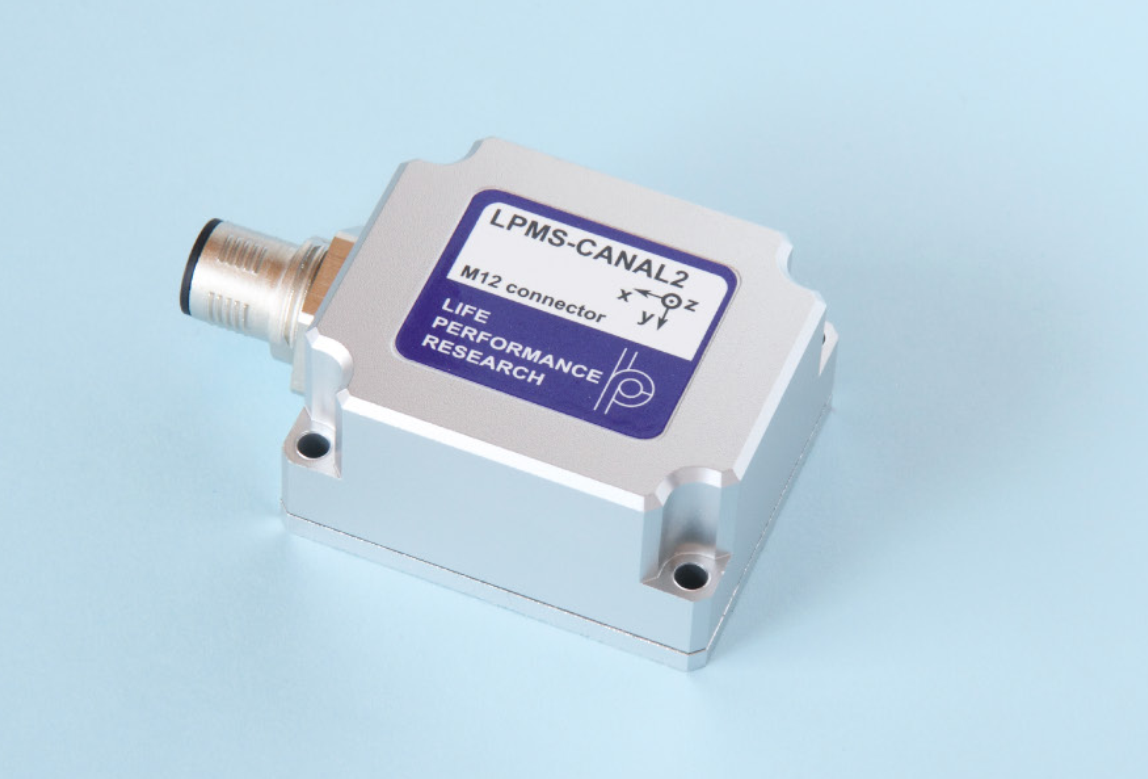
\includegraphics[width = 0.5\textwidth]{fig/tly.png}
	\caption{Alubi LPMS-CANAL2 陀螺仪}
	\label{tly}
\end{figure}

由产品手册总结得出陀螺仪信号处理流程:

\begin{figure}[H]
	\centering
	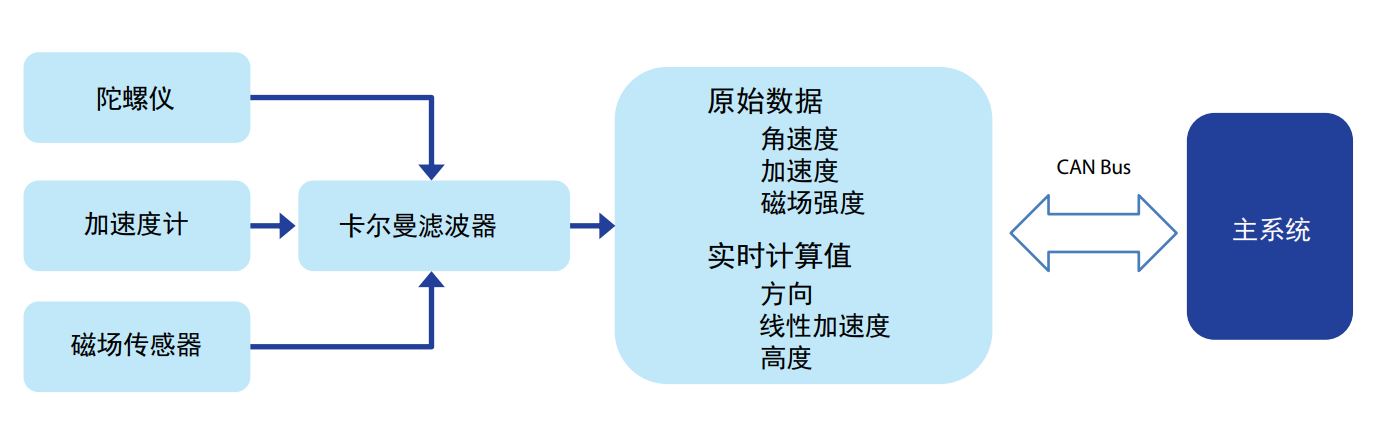
\includegraphics[width = 1\textwidth]{fig/tly_pipeline.png}
	\caption{陀螺仪信号处理信号}
	\label{tly_pipeline}
\end{figure}

光学传感器确定为\emph{CORREVIT® SFII P Optical Sensor}。它重量仅需250 g,开发用于测量轮胎打滑角度,并且应用了先进的DSP技术,主要通信接口为CAN Bus, RS232, USB。

\begin{figure}[H]
	\centering
	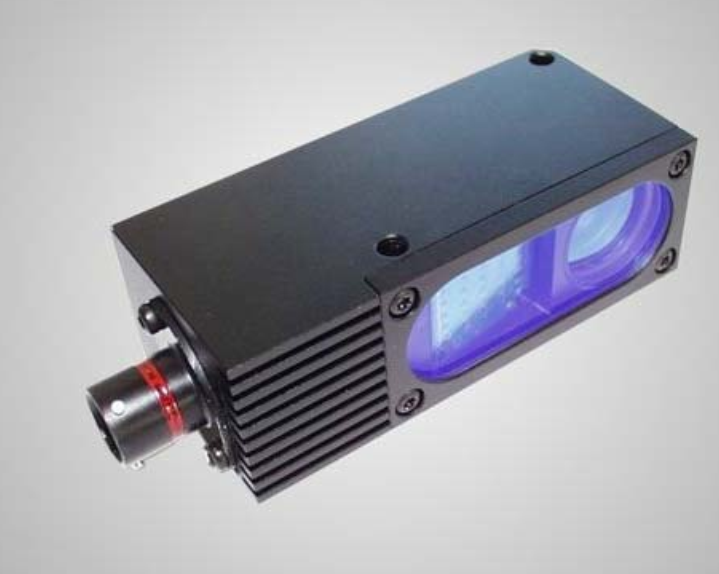
\includegraphics[width = 0.4\textwidth]{fig/gxcgq.png}
	\caption{CORREVIT® SFII P Optical Sensor}
	\label{gxcgq}
\end{figure}

%—————————(3)其他传感器:超声波传感器、惯导元件——————————

\textbf{(3) 其他传感器}

\begin{table}[H]
	\centering%表格居中
	\caption[centering]{其他传感器需求}%表格标题
	\label{qtxq}%表格标签
	\begin{tabular}{C{2cm}C{3cm}p{3cm}p{4cm}}	
		\toprule
		\tabincell{c}{\textbf{传感器}} &\tabincell{c}{\textbf{工况}} &\tabincell{c}{\textbf{功能}} &\tabincell{c}{\textbf{注意事项及要求}}\\ 
		\midrule
		
		\textbf{超声波传感器} & 2或多个,布置于侧方 & 发射接收超声波测量周围障碍 & 供电电压必须小于24V,且越小越好;尺寸要尽量小、测量精度要高;有良好封装 \\
		\\
		\textbf{惯导元件} & 1个非必须,布置于车身中部 & 实时测量车子运动学参数,作为动态控制算法的必要参数 & 测量延迟要小,精度要高 \\		
		
		\bottomrule
	\end{tabular}
\end{table}

其他传感器一般作为特殊功用时的补充,因此无具体选择型号。

\subsubsection{执行电机}

相关基础需求如下所示:

\begin{table}[H]
	\centering%表格居中
	\caption[centering]{电机需求}%表格标题
	\label{motorxq}%表格标签
	\begin{tabular}{C{2cm}C{3cm}p{3cm}p{4cm}}	
		\toprule
		\tabincell{c}{\textbf{电机}} &\tabincell{c}{\textbf{工况}} &\tabincell{c}{\textbf{功能}} &\tabincell{c}{\textbf{注意事项及要求}}\\ 
		\midrule
		
		\textbf{底盘驱动电机} & 四个布置于轮边 & 输出驱动扭矩,实现底盘运动 & 供电电压必须小于24V,且越小越好;输出扭力大 \\
		\\
		\textbf{云台yaw轴电机} & 1个布置于云台滑环处 & 输出驱动扭矩,实现云台运动 & 供电电压必须小于24V,输出扭力大;体积不限 \\		
		
		\bottomrule
	\end{tabular}
\end{table}

最终底盘电机电调确定为\emph{DJI M3508}为直流无刷减速电机,减速比为 19:1。该电机自带位置传感器,可提供位置反馈;还带有温度检测传感器,可防止电机被烧坏。 C620 电调支持 PWM 信号控制和 CAN 总线两种控制方式。

\begin{figure}[H]
	\centering
	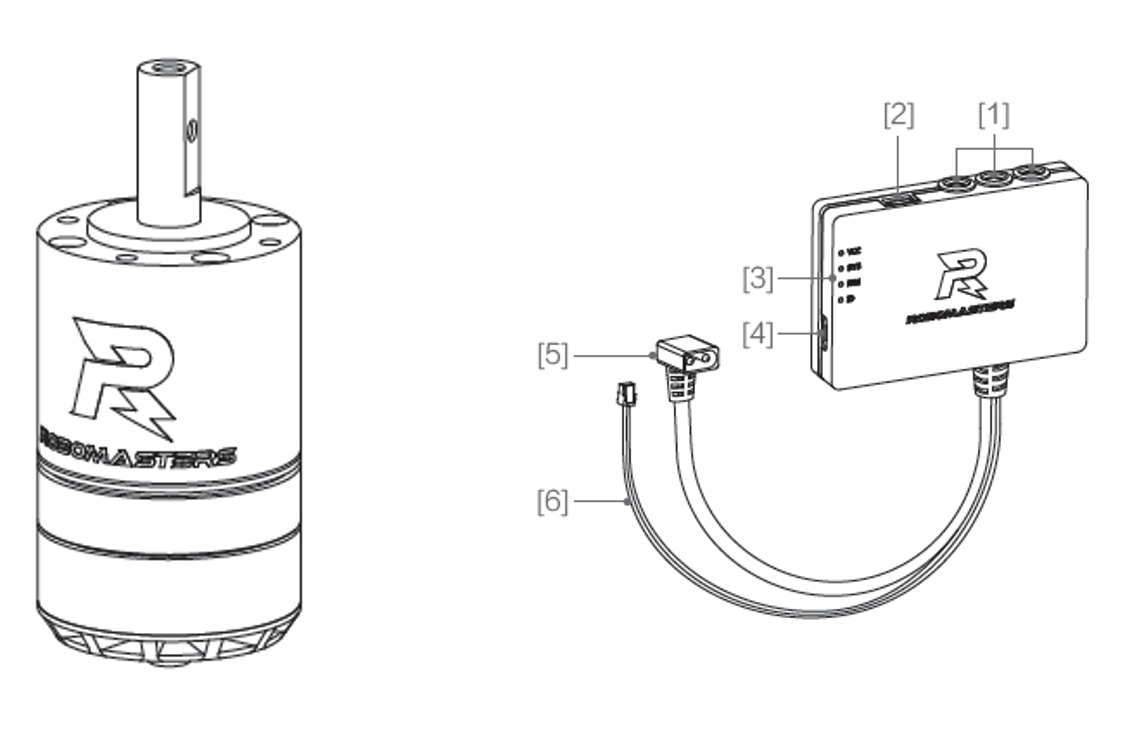
\includegraphics[width = 0.6\textwidth]{fig/3510.png}
	\caption{3510电机及其适配电调}
	\label{3510}
\end{figure}

3510电机及其适配电调示意如上图,其中电调较为重要的端口如下:

[1] 三相端口包含红色、黄色和黑色三个端口,必须匹配相应颜色连接RM 3510 减速电机的三相接头至该端口。

[2] 霍尔端口为RM 3510 减速电机内部的霍尔元件提供电源,并反馈霍尔元件的信号至电调。

[6] CAN 信号线连接至中心转接板的CAN 端口以接入CAN 总线。红线为CANH,黑线为CANL。根据协议规范,CAN 总线上需要接入两个120Ω 终端电阻,820R 电调已内置该电阻,用户可通过拨码开关选择是否接入。

此外,[3] LED 指示灯用于指示电调的不同状态;[4] Micro USB端口连接该端口至PC,使用RM 电调助手升级固件;[5] 电源线连接至中心转接板上的XT30 端口,通过中心转接板为电调供电



\subsubsection{中央处理器}

相关基础需求如下所示:

\begin{table}[H]
	\centering%表格居中
	\caption[centering]{中央处理器需求}%表格标题
	\label{cpuxq}%表格标签
	\begin{tabular}{C{2cm}C{3cm}p{3cm}p{4cm}}	
		\toprule
		\tabincell{c}{\textbf{处理器}} &\tabincell{c}{\textbf{工况}} &\tabincell{c}{\textbf{功能}} &\tabincell{c}{\textbf{注意事项及要求}}\\ 
		\midrule
		
		\textbf{中央处理器} & 1到2个布置于车身后部或车身内 & 整车采集数据的计算与指令决策的输出 & 供电电压必须小于24V,且越小越好;利于散热;有良好封装 \\
		
		\bottomrule
	\end{tabular}
\end{table}

最终选型是来自 Nvidia 的计算处理器板\emph{NVIDIA Jetson TX2},该处理器集成了 ARM 架构中央处理单元(CPU)。=相较于前代产品,Jetson TX2所提供的性能为早前版本的两倍,即能够以两倍以上的功效运行,且功率低于7.5瓦。这使得Jetson TX2能够在终端应用上运行更庞大、更深度的神经网络,让设备更加智能,具有更高的精度和更快的响应时间,以执行如图像分类、导航和语音识别等任务。该开发模块适合机器人、无人机、智能摄像机和便携医疗设备等智能终端设备。

根据\emph{jetson tx2 module datasheet v1.1}产品手册可以了解到,该板载计算机具有丰富的接口,包括USB,PCI Express,Serial Peripheral Interface,IIC, UART, CAN, JTAG等已知所有主流微机总线,较为方便进行智能机器人在感知、处理、决策等各方面的开发。

\begin{figure}[H]
	\centering
	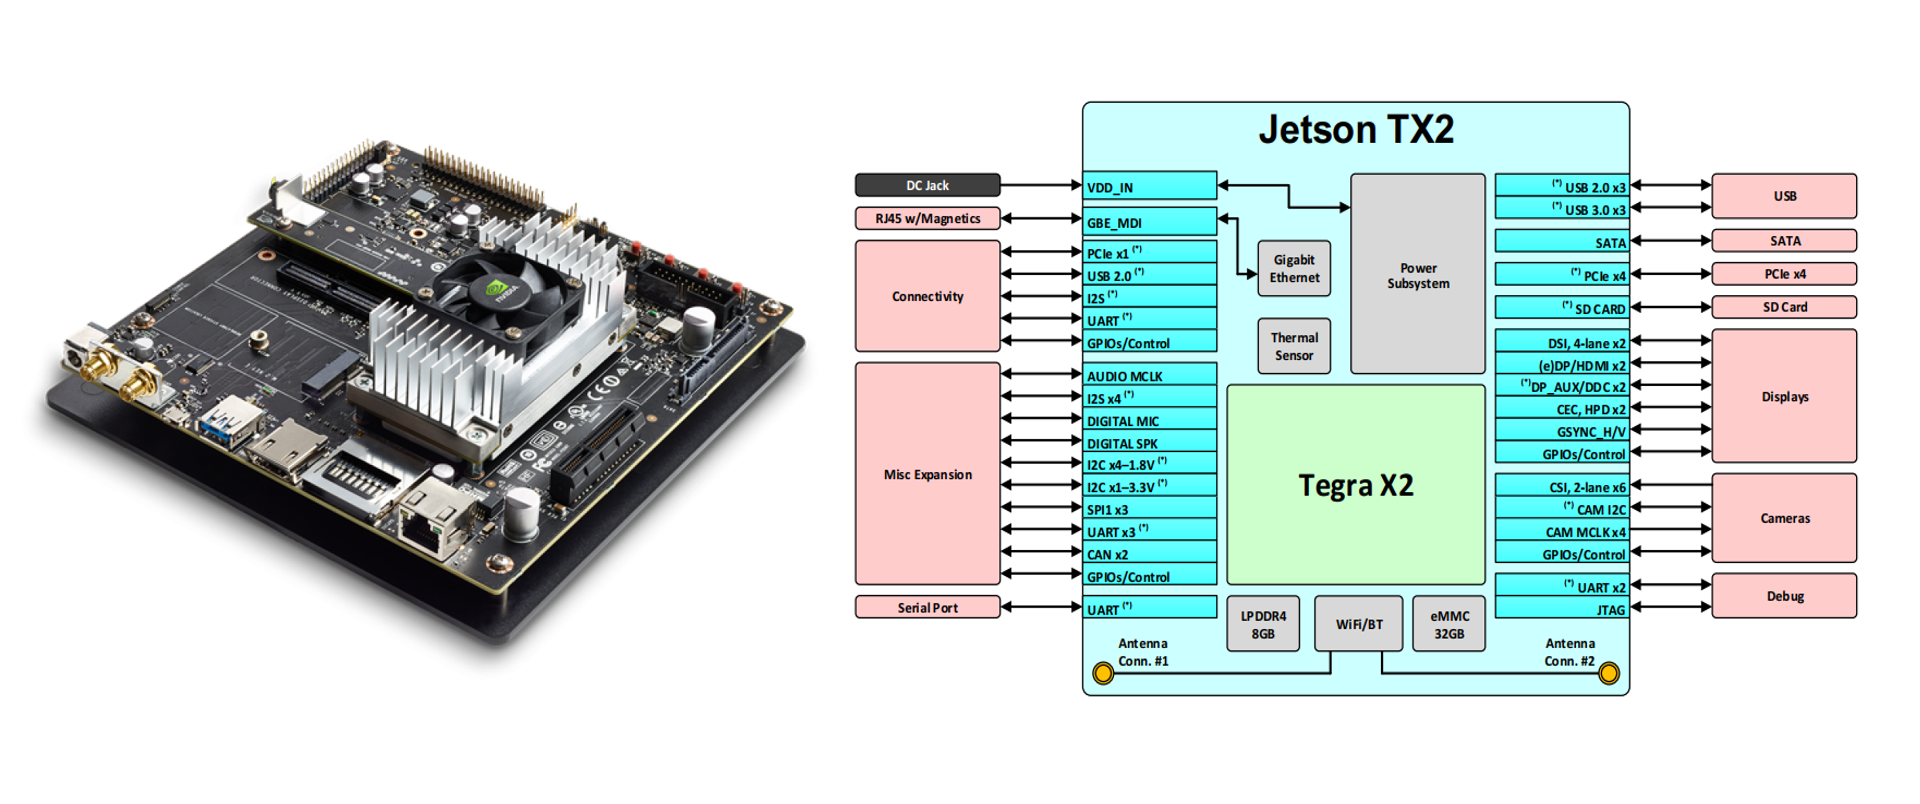
\includegraphics[width = 1\textwidth]{fig/tx_2.png}
	\caption{NVIDIA Jetson TX2实物与框图}
	\label{tx2}
\end{figure}

\subsubsection{传感器选择终选}

\begin{table}[H]
	\centering%表格居中
	\caption[centering]{电子电气最终选型}%表格标题
	\label{dzdqzu}%表格标签
	\begin{tabular}{C{2cm}C{3cm}C{5cm}C{3cm}}	
		\toprule
		\tabincell{c}{\textbf{功能}} &\tabincell{c}{\textbf{电子元件}} &\tabincell{c}{\textbf{通讯设备或协议}} &\tabincell{c}{\textbf{产品型号}}\\ 
		\midrule
		
		\textbf{中心主控} & 开发计算平台 & CAN, UART, IIC, USB, PCIe等 & NVIDIA Jetson TX2\\
		\textbf{底盘移动} & 直流无刷电机电调 & CAN或UART等 & DJI M3508+C620 \\
		\textbf{云台旋转} & 直流无刷电机电调 & CAN或UART等 & DJI EC60 \\
		\textbf{三维建图} & 双目摄像头 & USB & ZED \\
		& LiDAR\&GPS & 以太网, USB, UART & Hesai Pandar 40 \\
		\textbf{自主避障} & 超声波模块 & GPIO & HC-SR04 \\
		\textbf{状态检测} & 陀螺仪 & IIC & Alubi LPMS-CANAL2 \\
		& IMU & CAN, USB等\\
		\bottomrule
	\end{tabular}
\end{table}

\subsection{总线框架设计}

AtomIC总线布置方面,最主要的就是CAN总线技术,其次是IIC、SBUS串口和USART。

在工业场合应用上,尤其是车辆电气架构上,CAN保证不会在出现在RS-485网络中的现象,即当系统有错误,出现多节点同时向总线发送数据时,导致总线呈现短路,从而损坏某些节点的现象。而且CAN节点在错误严重的情况下具有自动关闭输出功能,以使总线上其他节点的操作不受影响,从而保证不会出现像在网络中,因个别节点出现问题,使得总线处于“死锁”状态。而且,CAN具有的完善的通信协议可由CAN控制器芯片及其接口芯片来实现,从而大大降低系统开发难度,缩短了开发周期,这些是仅有电气协议的RS-485所无法比拟的。

出于稳定性考虑,CAN总线技术为重要协议。并且因为DJI提供的820R底盘电机电调和6623号云台轴电机都是对外提供CAN接口的。通过CAN总线将主控、云台和底盘进行串联,布线简单,既能向每一个ID的电机输入特定的信号,又能解析出每个特定电机的返回值(码盘值或者速度值)。除了主控-云台-底盘的CAN总线系统之外,AtomIC平台还使用了CAN2系统,用以预留其他电机的接口应用。

至于I2C,在所选定陀螺仪中,陀螺仪读值是通过I2C总线传给主控的CPU进行解算的;SBUS协议主要用于遥控器接收机与主控DMA之间的通信,以达到遥控AtomIC的目的;USART主要用于串口通信,用于如GPS信号、超声波信号与上位机进行数据互换的功用。